\documentclass[12pt]{report}
\usepackage{placeins}
% -------- Idioma primero --------
\usepackage[english,shorthands=off]{babel}
\usepackage{csquotes}

% -------- Fuentes para LuaLaTeX --------
\usepackage{fontspec}
\defaultfontfeatures{Ligatures=TeX}
\setmainfont{Latin Modern Roman}
\setmonofont{DejaVu Sans Mono}[Scale=MatchLowercase]

% -------- Maquetación y utilidades --------
\usepackage{geometry}
\geometry{a4paper, margin=2.5cm}
\usepackage{graphicx}
\usepackage{amsmath,amssymb,mathtools}
\usepackage{xcolor}
\usepackage{soul}
\definecolor{mylime}{HTML}{CCFF00} % opcional: “lime” seguro
\sethlcolor{mylime}
\usepackage{booktabs}
\usepackage{tabularx}
\usepackage{array}
\usepackage{longtable}
\usepackage{svg}
\usepackage{csvsimple}

\usepackage{xspace}
\newcommand{\LCOW}{\textsc{LCOW}\xspace}

\usepackage{siunitx}
\sisetup{
  output-decimal-marker = {,}, % coma decimal
  group-separator       = {.}, % punto de miles
  group-minimum-digits  = 3,
  reset-text-series     = false,
  text-series-to-math   = true
}

\usepackage{makecell}
\renewcommand\theadfont{\bfseries}

\usepackage{newunicodechar}
\newunicodechar{≥}{\ensuremath{\ge}}
\newunicodechar{≤}{\ensuremath{\le}}
\newunicodechar{↕}{\ensuremath{\updownarrow}}

\usepackage{threeparttable}
\usepackage[ruled,vlined]{algorithm2e}

% Si mantienes esto, ya no hace falta, pero no molesta:
\AtBeginDocument{\shorthandoff{"<>.!}}

% -------- BibLaTeX + APA (Biber) --------
\usepackage[backend=biber,
            style=apa,
            citestyle=authoryear,
            maxcitenames=2,
            uniquelist=false,
            sorting=nyt]{biblatex}
\addbibresource{referencias.bib}

% -------- Título del abstract --------
\addto\captionsspanish{\renewcommand{\abstractname}{Abstract}}

% -------- Entorno abstract sin índice --------
%\makeatletter
%\renewenvironment{abstract}{%
%  \chapter*{\abstractname}%
%  \markboth{\abstractname}{\abstractname}%
%}{}
%\makeatother

% -------- Siempre al final --------
\usepackage{hyperref}
\hypersetup{hidelinks}

\title{Ideational Bricoleurs in Forest Adaptation Governance: Germany--Chile Comparison}
\author{Aharon Esteban Valdés-Zúñiga \\ Global Studies Programme \\ University of Freiburg}
\date{\vspace{-5ex}}

\begin{document}
\sloppy

% ======= Front matter en romanos desde el inicio =======
\pagenumbering{roman}
\setcounter{page}{1}

% -------- Portada --------
\begin{titlepage}
  \thispagestyle{empty}
  \centering

  {\LARGE \textsc{Albert Ludwig University of Freiburg}\par}
  \vspace{0.5em}
  {\Large \textsc{Global Studies Programme}\par}
  \vspace{0.25em}
  {\large \textsc{Thesis Proposal}\par}

  \vspace{3cm}
  {\huge\bfseries Discourse and Institutional Bricolage in Forest Adaptation Governance: A Comparative Study of Germany and Chile \par}

  \vspace{2cm}
  {\Large Author: Aharon Esteban Valdés-Zúñiga\par}

  \vfill
  {\large Freiburg im Breisgau, Germany\par}
  {\large \today\par}
\end{titlepage}



% -------- Resumen --------
% --- Resumen / Abstract ---
\begin{abstract}
How do actors in contrasting institutional contexts assemble discourses and
instruments for forest adaptation, and how far do their ideas travel? This
thesis compares Germany and Chile as most-different cases of forest governance.
Building on discursive institutionalism and the concept of \emph{ideational
bricolage}, it introduces an \textbf{Uptake Index} to trace how frames and
instruments circulate across policy arenas. The study analyzes a corpus of
50--60 key documents (2015--2025) through systematic coding. It is expected
that (1) Germany’s dense institutional setting fosters incremental layering of
established tools, while (2) Chile’s fragmented governance encourages
transposition and more radical recombination. These dynamics generate distinct
uptake profiles across the two cases. The contribution is twofold: theoretically,
by clarifying mechanisms of discursive translation; and methodologically, by
offering a replicable tool for assessing policy uptake.
\\
\\
\noindent\textbf{Keywords:} forest adaptation, discursive institutionalism,
ideational bricolage, Uptake Index, Germany, Chile, policy uptake
\end{abstract}


% -------- Índice --------
\clearpage
\renewcommand{\contentsname}{Index}
\tableofcontents

% ======= Cuerpo en arábigos =======
\clearpage
\pagenumbering{arabic}
\setcounter{page}{1}

% -------- Cuerpo --------
% ================================
% Introduction
% ================================

\section*{Introduction}
\addcontentsline{toc}{section}{Introduction}

Forests are at the frontline of the climate crisis: simultaneously vital carbon
sinks and highly vulnerable ecosystems. Intensifying droughts, wildfires, and
pest outbreaks are transforming forests from buffers into emission sources. In
Germany, four out of five trees were classified as diseased in 2022 due to
drought and bark beetle infestations (\cite{BMEL2023}); in Chile, a decade-long
\emph{megasequía} combined with record wildfires has placed immense stress on
both native ecosystems and plantation economies (\cite{FAO2022}). Policy
responses increasingly foreground adaptation, from Germany’s
\emph{Waldstrategie 2050} to Chile’s \emph{Plan Nacional de Restauración de
Paisajes 2021–2030} (\cite{MMA2021}). Yet little is known about
\emph{how} actors in such divergent contexts recombine discursive and
institutional elements, or how their ideas circulate across policy arenas.

Existing research emphasizes the role of institutions in shaping responses to
forest decline (\cite{Winkel2011}; Winkel \& Sotirov 2016) and the power of ideas
in legitimizing adaptation pathways (\cite{Schmidt2008}). However, less attention
has been paid to how actors strategically \emph{combine} discursive frames and
institutional instruments. Discursive institutionalism highlights the power of
ideas \emph{in, through, and over} institutions, while the notion of
\emph{ideational bricolage} underscores how actors recombine heterogeneous
resources into workable strategies. Integrating these perspectives allows for a
sharper theorization of adaptation governance.

This thesis adopts a comparative design. Germany represents a dense corporatist
context where adaptation is typically layered onto existing institutions, while
Chile exemplifies a fragmented neoliberal system where bricolage often proceeds
through transposition or novel assemblages. By tracing actors’ discursive
strategies and their observable uptake, the study explains how contrasting
governance logics shape the forms of bricolage available.

The contribution is threefold: (i) theoretical, by integrating discursive
institutionalism and bricolage into a causal framework; (ii) methodological, by
operationalizing bricolage through a transparent Uptake Index; and (iii)
empirical, by adding a Global South case to a research field dominated by
Northern perspectives. 
\section*{Research Questions}
\begin{quote}
\textbf{RQ1 (primary).} Under what institutional conditions do actors engage in 
\emph{ideational bricolage} in forest adaptation governance?  

\textbf{RQ2 (secondary).} What specific forms of \emph{uptake} (textual reuse, funding allocation, 
institutional incorporation, representation) result from such bricolage across policy arenas?  
\end{quote}

\section*{Hypotheses}
\begin{itemize}
  \item \textbf{H1.} In dense institutional contexts (Germany), bricolage manifests as layering/patching, 
  with uptake clustered in textual reuse and institutional incorporation.  
  \item \textbf{H2.} In fragmented contexts (Chile), bricolage manifests as transposition/assemblage, 
  with uptake clustered in funding allocations and venue representation.  
  \item \textbf{H3.} Actor type conditions bricolage: NGOs combine justice-based frames with ecological claims; 
  industry combines efficiency/productivity with market instruments.  
\end{itemize}

\section*{Case Justification}
Germany and Chile are selected as a most-different systems design. Both face analogous biophysical threats 
(droughts, wildfires, forest dieback) but are embedded in sharply contrasting political–institutional contexts. 
Germany exemplifies dense corporatism; Chile, fragmented neoliberalism. This contrast maximizes analytical leverage 
and avoids Eurocentric bias.
% ================================
% Propositions
% ================================

\section*{Propositions}
\addcontentsline{toc}{section}{Propositions}

The propositions extend prior literature but introduce a novel dimension: for the 
first time, uptake is measured systematically with a replicable \textbf{Uptake Index}. 
This enables testing not only whether bricolage differs across contexts, but also 
how discursive recombinations translate into measurable governance outcomes.

\begin{itemize}
    \item \textbf{P1: Institutional density conditions bricolage modes.}  
    In contexts of high institutional density (Germany), bricolage will manifest 
    primarily as layering or patching. In fragmented contexts (Chile), bricolage 
    will manifest more often as transposition or novel assemblages.  
    \textit{Novelty:} Unlike prior descriptive claims, this proposition will be tested 
    by comparing Uptake Index clustering patterns across cases.

    \item \textbf{P2: Actor type shapes discursive recombination.}  
    NGOs combine justice/rights frames with ecological claims, while industry 
    combines efficiency/productivity with market instruments.  
    \textit{Novelty:} The Uptake Index disaggregates how these recombinations travel 
    through different uptake channels (representation vs. funding vs. textual reuse).

    \textit{Illustrative example:} In the Chilean context, proposals linking 
    forest certification schemes with indigenous community councils could 
    hypothetically exemplify transposition bricolage. This remains to be 
    tested empirically in the coding stage, but illustrates how the concept 
    differs from policy entrepreneurship (focused on agenda timing) or 
    discourse coalitions (focused on storyline stabilization).

    \item \textbf{P3: Venue strategy influences uptake pathways.}  
    Actors targeting low-veto venues (advisory councils, certification) will achieve 
    higher uptake than those targeting high-veto venues (parliamentary arenas).  
    \textit{Novelty:} This is the first attempt to quantify venue effects using a 
    standardized uptake metric.
\end{itemize}

\subsection*{Comparative Strategy}

The research design follows a structured-focused comparison:  
\textit{structured}, because each actor type is examined with the same set of guiding questions;  
\textit{focused}, because the questions derive directly from the conceptual framework.  
This ensures comparability while preserving contextual specificity.

For each actor type (state, NGOs, business, science) in Germany and Chile, the analysis asks:

\begin{enumerate}
    \item Which discursive frames are mobilized? 
    \item Which institutional instruments are invoked? 
    \item How are these elements recombined (layering, patching, transposition, novel assemblage)? 
    \item Which governance venues are targeted? 
    \item What observable uptake can be identified? 
\end{enumerate}

This design prevents the analysis from devolving into parallel narratives. 
Instead, it enables systematic comparison of bricolage practices across institutional contexts, 
highlighting not whether Chile deviates from Germany, but how different governance logics 
produce distinct forms of bricolage and uptake.

\paragraph{Novelty.} 
These propositions are not mere extensions of prior literature: they operationalize 
\emph{uptake} for the first time with a replicable index. No existing study has systematically 
tested bricolage across North–South contexts with a standardized Uptake Index (so far). 
This makes the contribution both theoretical and methodological.
% ================================
% Literature Review
% ================================

\section*{Literature Review}
\addcontentsline{toc}{section}{Literature Review}

\subsection*{Concepts and Theoretical Approaches}

Understanding the politics of forest adaptation requires connecting 
\emph{discursive institutionalism} (DI) with the pragmatics of \emph{institutional bricolage}.  

First, DI highlights how institutions are simultaneously material and ideational, 
carrying discourses that give them meaning \parencite{Schmidt2008}. The distinction 
between \textit{coordinative} discourse (among elites) and \textit{communicative} 
discourse (towards publics) clarifies adaptation debates. The related concept of 
\emph{ideational power} specifies mechanisms of influence—persuasive power through ideas, 
power over which ideas are legitimate, and institutional power embedded in rules 
\parencite{CarstensenSchmidt2016}.

Second, bricolage explains the \textit{how} of recombination. Initially developed by 
L\'{e}vi-Strauss, the concept was adapted to natural resource governance to describe 
how actors pragmatically patch together rules, norms, and practices under constraint 
\parencite{Cleaver2001,Carstensen2017}. Bricolage is particularly visible in times of 
crisis or institutional voids.

Bringing DI and bricolage together highlights the figure of the 
\textbf{ideational bricoleur}: an actor who recombines discursive frames and 
institutional instruments into workable strategies. This bridges macro-level 
discursive struggles with micro-level practices of recombination. 

Alternative frameworks—policy entrepreneurship \parencite{Kingdon1995}, epistemic 
communities \parencite{Haas1992}, discourse coalitions \parencite{Hajer1995}—inform 
specific dynamics of agency but do not explain how heterogeneous elements are 
recombined into new institutional arrangements. They remain auxiliary lenses here.

\subsection*{Empirical Updates in Forest Adaptation (2020--2024)}



In Germany, the \textit{Report of the Scientific Advisory Board on Forest Policy} 
(Thünen Institute, 2022) outlines adaptation pathways and governance challenges. 
The European Forest Institute review by Verkerk et al. (2022) synthesizes 
evidence on climate disturbances and policy instruments. Winkel et al. (2022) 
analyze multifunctionality discourses in EU policy, while the \textit{Forest Europe 
Implementation Report} (2021--2024) compares national trajectories.  

In Chile, the World Bank (2023) positions forests as pillars of sustainable growth, 
linking adaptation to social inclusion. National initiatives include the 
\emph{Plan Nacional de Restauración de Paisajes 2021--2030} \parencite{MMA2021} and 
the \emph{Ecosystem Restoration Country Dossier} \parencite{MMACONAF2024}. 
Scientific contributions emphasize wildfire dynamics \parencite{VidalSilva2025}, 
forest hydrology \parencite{Balocchi2023}, and biodiversity restoration 
\parencite{Bosque2022Biodiversity,RCHN2023Restoration}. These highlight both 
biophysical urgency and institutional fragmentation.

\subsection*{Forest Governance and Adaptation Studies}

European scholarship emphasizes the institutionalization of discourses 
\parencite{ArtsBuizer2009,Winkel2011}, certification and non-state authority 
\parencite{Cashore2004}, and multi-level policy interaction 
\parencite{Pulzl2013}. German adaptation discourses remain path-dependent, layered 
onto long-standing forestry–conservation conflicts \parencite{Winkel2011}.  

In Latin America, forest governance is marked by tenure insecurity, privatization, 
and contestation of extractive models \parencite{LarsonRibot2007,Manuschevich2016}. 
Critical perspectives stress neoliberal legacies and indigenous struggles 
\parencite{Gudynas2011,Escobar1996}. Chile illustrates how plantation-centered 
institutions shape adaptation discourses in tension with territorial rights.

Latin American scholarship further highlights community-based adaptation and 
indigenous rights (e.g., Boelens 2016; Oyarzún 2021; Banwell 2022), broadening 
the perspective beyond state-centered accounts.

\subsection*{Identified Gap and Justification}

Despite advances, no comparative research systematically examines the 
\textbf{ideational bricoleur} as a mechanism in North–South forest adaptation governance.  
Existing studies document discursive struggles in Europe \parencite{Winkel2011}, 
institutional fragmentation in Chile \parencite{Manuschevich2016}, and recent 
scholarship links adaptation to governance scales 
\parencite{Kleinschmit2024,KleinschmitChiassonPulzl2023}.  

Yet the specific micro-practices by which actors recombine discursive and 
institutional elements—and how these generate observable uptake—remain untheorized.  
This thesis addresses that gap by integrating DI and bricolage through the concept 
of the ideational bricoleur, applying it systematically in a most-different systems 
comparison of Germany and Chile.

\begin{table}[h!]
\centering
\tiny
\caption{Selected literature on forest adaptation governance, bricolage, and discourse}
\label{tab:litreview}
\begin{tabular}{@{}p{2.5cm}p{2.5cm}p{3cm}p{4cm}p{4.5cm}@{}}
\toprule
\textbf{Author, Year} & \textbf{Concept} & \textbf{Context} & \textbf{Method} & \textbf{Key Findings} \\ \midrule
Winkel (2011) & Discursive institutionalism & Germany & Frame analysis & Discursive struggles drive governance; path dependency in adaptation debates. \\
Manuschevich (2016) & Neoliberal legacies & Chile & Policy/legal analysis & Fragmented institutions constrain adaptation; plantation model dominates. \\
Pahl-Wostl (2015) & Institutional bricolage & Comparative water governance & Case studies & Typology of layering/patching/transposition; informs coding. \\
Mukhtarov (2014) & Policy translation & Europe/global & Discourse analysis & Shows how concepts travel; relevant for Uptake Index. \\
Carstensen \& Schmidt (2016) & Ideational power & Europe & Theory synthesis & Specifies mechanisms of ideational influence; supports DI link. \\
Boelens (2016) & Community water governance & Latin America & Comparative ethnography & Highlights indigenous rights, collective adaptation, bricolage practices. \\
Kleinschmit et al. (2023, 2024) & Multilevel forest governance & EU/Chile & Policy analysis & Emphasize scale interactions and adaptation governance. \\
\bottomrule
\end{tabular}
\end{table}
% ================================
% Conceptual Framework
% ================================

\section*{Conceptual Framework}
\addcontentsline{toc}{section}{Conceptual Framework}

\subsection*{Positioning the Concept of the Ideational Bricoleur}

The central conceptual contribution of this thesis is the specification of the 
\textit{ideational bricoleur}. This figure links discursive frames 
(diagnostic, prognostic, motivational) with institutional recombination 
(layering, patching, transposition) and observable uptake 
(textual reuse, funding allocation, institutional incorporation, representation). 
Discursive Institutionalism provides the macro logic of ideas in, through, and over 
institutions, while Institutional Bricolage specifies the micro practices of 
recombination. The analytical claim is that bricolage modes and their uptake 
systematically vary by institutional density and fragmentation.

\paragraph{Differentiation from adjacent concepts.}
The \textit{ideational bricoleur} is distinct from other well-established concepts.  
Unlike \textbf{policy entrepreneurs} \parencite{Kingdon1995}, whose defining feature is 
strategic coupling of problem, policy, and political streams, bricoleurs are 
identified by the substantive recombination of heterogeneous elements 
(e.g., legal instruments + scientific evidence + customary norms).  
Unlike \textbf{discourse coalition brokers} \parencite{Hajer1995}, who stabilize shared 
storylines across networks, bricoleurs operate at the junction of discourse and 
institutional practice, assembling fragments into workable arrangements.  

The added explanatory value lies in clarifying a mechanism that neither policy 
entrepreneurship nor discourse coalition theory makes visible: the translation of 
discursive frames into institutional instruments with empirically observable uptake.

\paragraph{Illustrative example.}
For instance, in Chile, proposals that combine international certification schemes 
with indigenous co-management councils exemplify \emph{ideational bricolage}. 
Such recombination differs from policy entrepreneurship (focused on agenda windows) 
and from discourse coalitions (focused on shared storylines), because it assembles 
heterogeneous instruments into a concrete governance design.

\paragraph{Analytical bridge.}
The bricoleur concept serves as a bridge, not a replacement. Policy entrepreneurship, 
epistemic communities, and discourse coalitions are employed only as auxiliary lenses 
to test boundary conditions; they are not part of the causal model. The explanatory 
focus rests squarely on bricolage as a mechanism of discursive translation into 
governance uptake. This delimitation prevents conceptual dilution while signaling 
awareness of adjacent frameworks.

\paragraph{Causal expectations.}
The framework predicts:  
\begin{itemize}
    \item In dense systems (Germany), bricolage will manifest primarily as layering 
    and patching, producing broader but incremental uptake.  
    \item In fragmented systems (Chile), bricolage will manifest more often as 
    transposition or novel assemblages, producing selective but more variable uptake.  
    \item Across cases, state actors will generally achieve higher uptake due to venue 
    access, but this gap will narrow in fragmented systems where NGOs and academics 
    substitute governance capacity.  
\end{itemize}

In sum, the \textit{ideational bricoleur} captures the micro-level practices through 
which discursive innovations are assembled into institutional proposals and tested in 
policy arenas. This provides a clear mechanism linking discourse, bricolage, and 
uptake, directly operationalized through the Uptake Index.


\paragraph{Contribution to broader debates.}
Beyond forest governance, this framework contributes to wider discussions in 
climate governance and North–South epistemologies by showing how ideas travel, 
hybridize, and gain uptake across highly divergent institutional contexts.
% ================================
% Methodology
% ================================

\section*{Methodology}
\addcontentsline{toc}{section}{Methodology}

\subsection*{Research Design}
This study applies a qualitative, theory-building comparative case study design 
\parencite{George2005}. Germany and Chile are selected as ``most different systems'': 
both face similar biophysical pressures (droughts, wildfires, forest dieback) but 
are embedded in sharply contrasting political–institutional contexts. This design 
maximizes analytical leverage by showing how divergent legacies condition actor strategies.

\textbf{Germany} represents a corporatist welfare state with dense institutions 
and a tradition of consensus-oriented forestry.  
\textbf{Chile} exemplifies a fragmented neoliberal system with powerful 
private-sector actors and persistent socio-environmental conflicts.  
Comparing the two illuminates how institutional density versus fragmentation 
shapes bricolage strategies and uptake.

\subsection*{Operationalizing Observable Uptake}
Effectiveness of bricolage is defined through \textbf{observable uptake} in governance processes.  
Four indicators are coded:

\begin{enumerate}
    \item \textbf{Textual reuse in official drafts or laws.} Evidence of frames/instruments 
    appearing verbatim or paraphrased in legislation, decrees, or strategies. 
    \item \textbf{Resource allocation.} Clear link between proposals and funding (subsidies, 
    grants, pilot initiatives). 
    \item \textbf{Institutional incorporation.} Inclusion of bricolage elements in agency 
    mandates, procedures, or reporting frameworks. 
    \item \textbf{Actor representation.} Proponents gain seats or speaking roles in 
    decision-making venues (hearings, councils, advisory bodies). 
\end{enumerate}

\paragraph{Uptake Index weights.}
These four dimensions are reported \emph{disaggregated} and as a simple cumulative score (0–4).  
The cumulative score summarizes breadth, but does not imply equivalence (e.g., a law ≠ a 
hearing seat). Robustness checks test weighted alternatives (laws = 2; funding = 1.5) 
and an ordinal intensity scale (0–2). This prevents spurious equivalence and shows that 
findings are not artifacts of the index specification.

\paragraph{Negative uptake.}
Negative uptake is coded when a frame/instrument is explicitly rejected in official 
texts (e.g., ``inadmissible'', ``incompatible with X''). Rejections are treated as 1 
on a separate variable, ensuring that counter-mobilization is visible.

\paragraph{Timing.}
A lag variable records months between proposal and uptake, adding granularity 
to the analysis of how quickly bricolage diffuses.

\subsection*{Identifying Ideational Bricoleurs}
An actor (organization, coalition, or individual) is coded as a bricoleur when 
three \emph{observable} conditions are met:

\begin{enumerate}
    \item \textbf{Discursive recombination:} explicit combination of at least two 
    frames (e.g., ecological + justice; market + rights). 
    \item \textbf{Institutional patching:} linking or adapting instruments from 
    different domains (e.g., certification + indigenous co-management). 
    \item \textbf{Solution-framing:} presence of prescriptive markers such as 
    ``we propose'', ``should be implemented'', ``this measure will'', ensuring 
    only explicit problem–solution couplings are coded. 
\end{enumerate}

This avoids guessing ``intent'' and anchors classification in textual evidence.  
Modes of bricolage (layering, patching, transposition) are coded separately.  
Actors are stratified by type (state, NGO, business, science) to ensure comparability.

\subsection*{Auxiliary Frameworks}
Policy entrepreneurship, epistemic communities, and discourse coalitions are used 
\emph{only as boundary checks}. For instance, if bricolage clusters around individuals 
exploiting agenda windows, this is noted in memos (policy entrepreneurship), or if 
expert networks explain uptake, this is flagged (epistemic communities). These frameworks 
are not part of the core causal model, avoiding conceptual dilution.

\subsection*{Corpus Construction}
The corpus covers 2015–2025.  

\textbf{Primary corpus (30–40 docs/country):} high-salience laws, strategies, 
policy briefs from state, NGO, and industry actors.  
\textbf{Secondary corpus:} grey literature/media for context (not systematically coded).  

Inclusion: explicit forest adaptation/governance content; Exclusion: purely 
technical reports or duplicates.  

Search terms: DE (``Waldstrategie'', ``Anpassung Forst'', ``Borkenkäfer''),  
ES (``adaptación forestal'', ``Plan Nacional de Restauración''),  
EN (``forest adaptation'', ``ecosystem restoration'').  

Final sample: $\sim$65 documents (see Figure~\ref{fig:prisma}).  

\begin{figure}[h!]
\centering
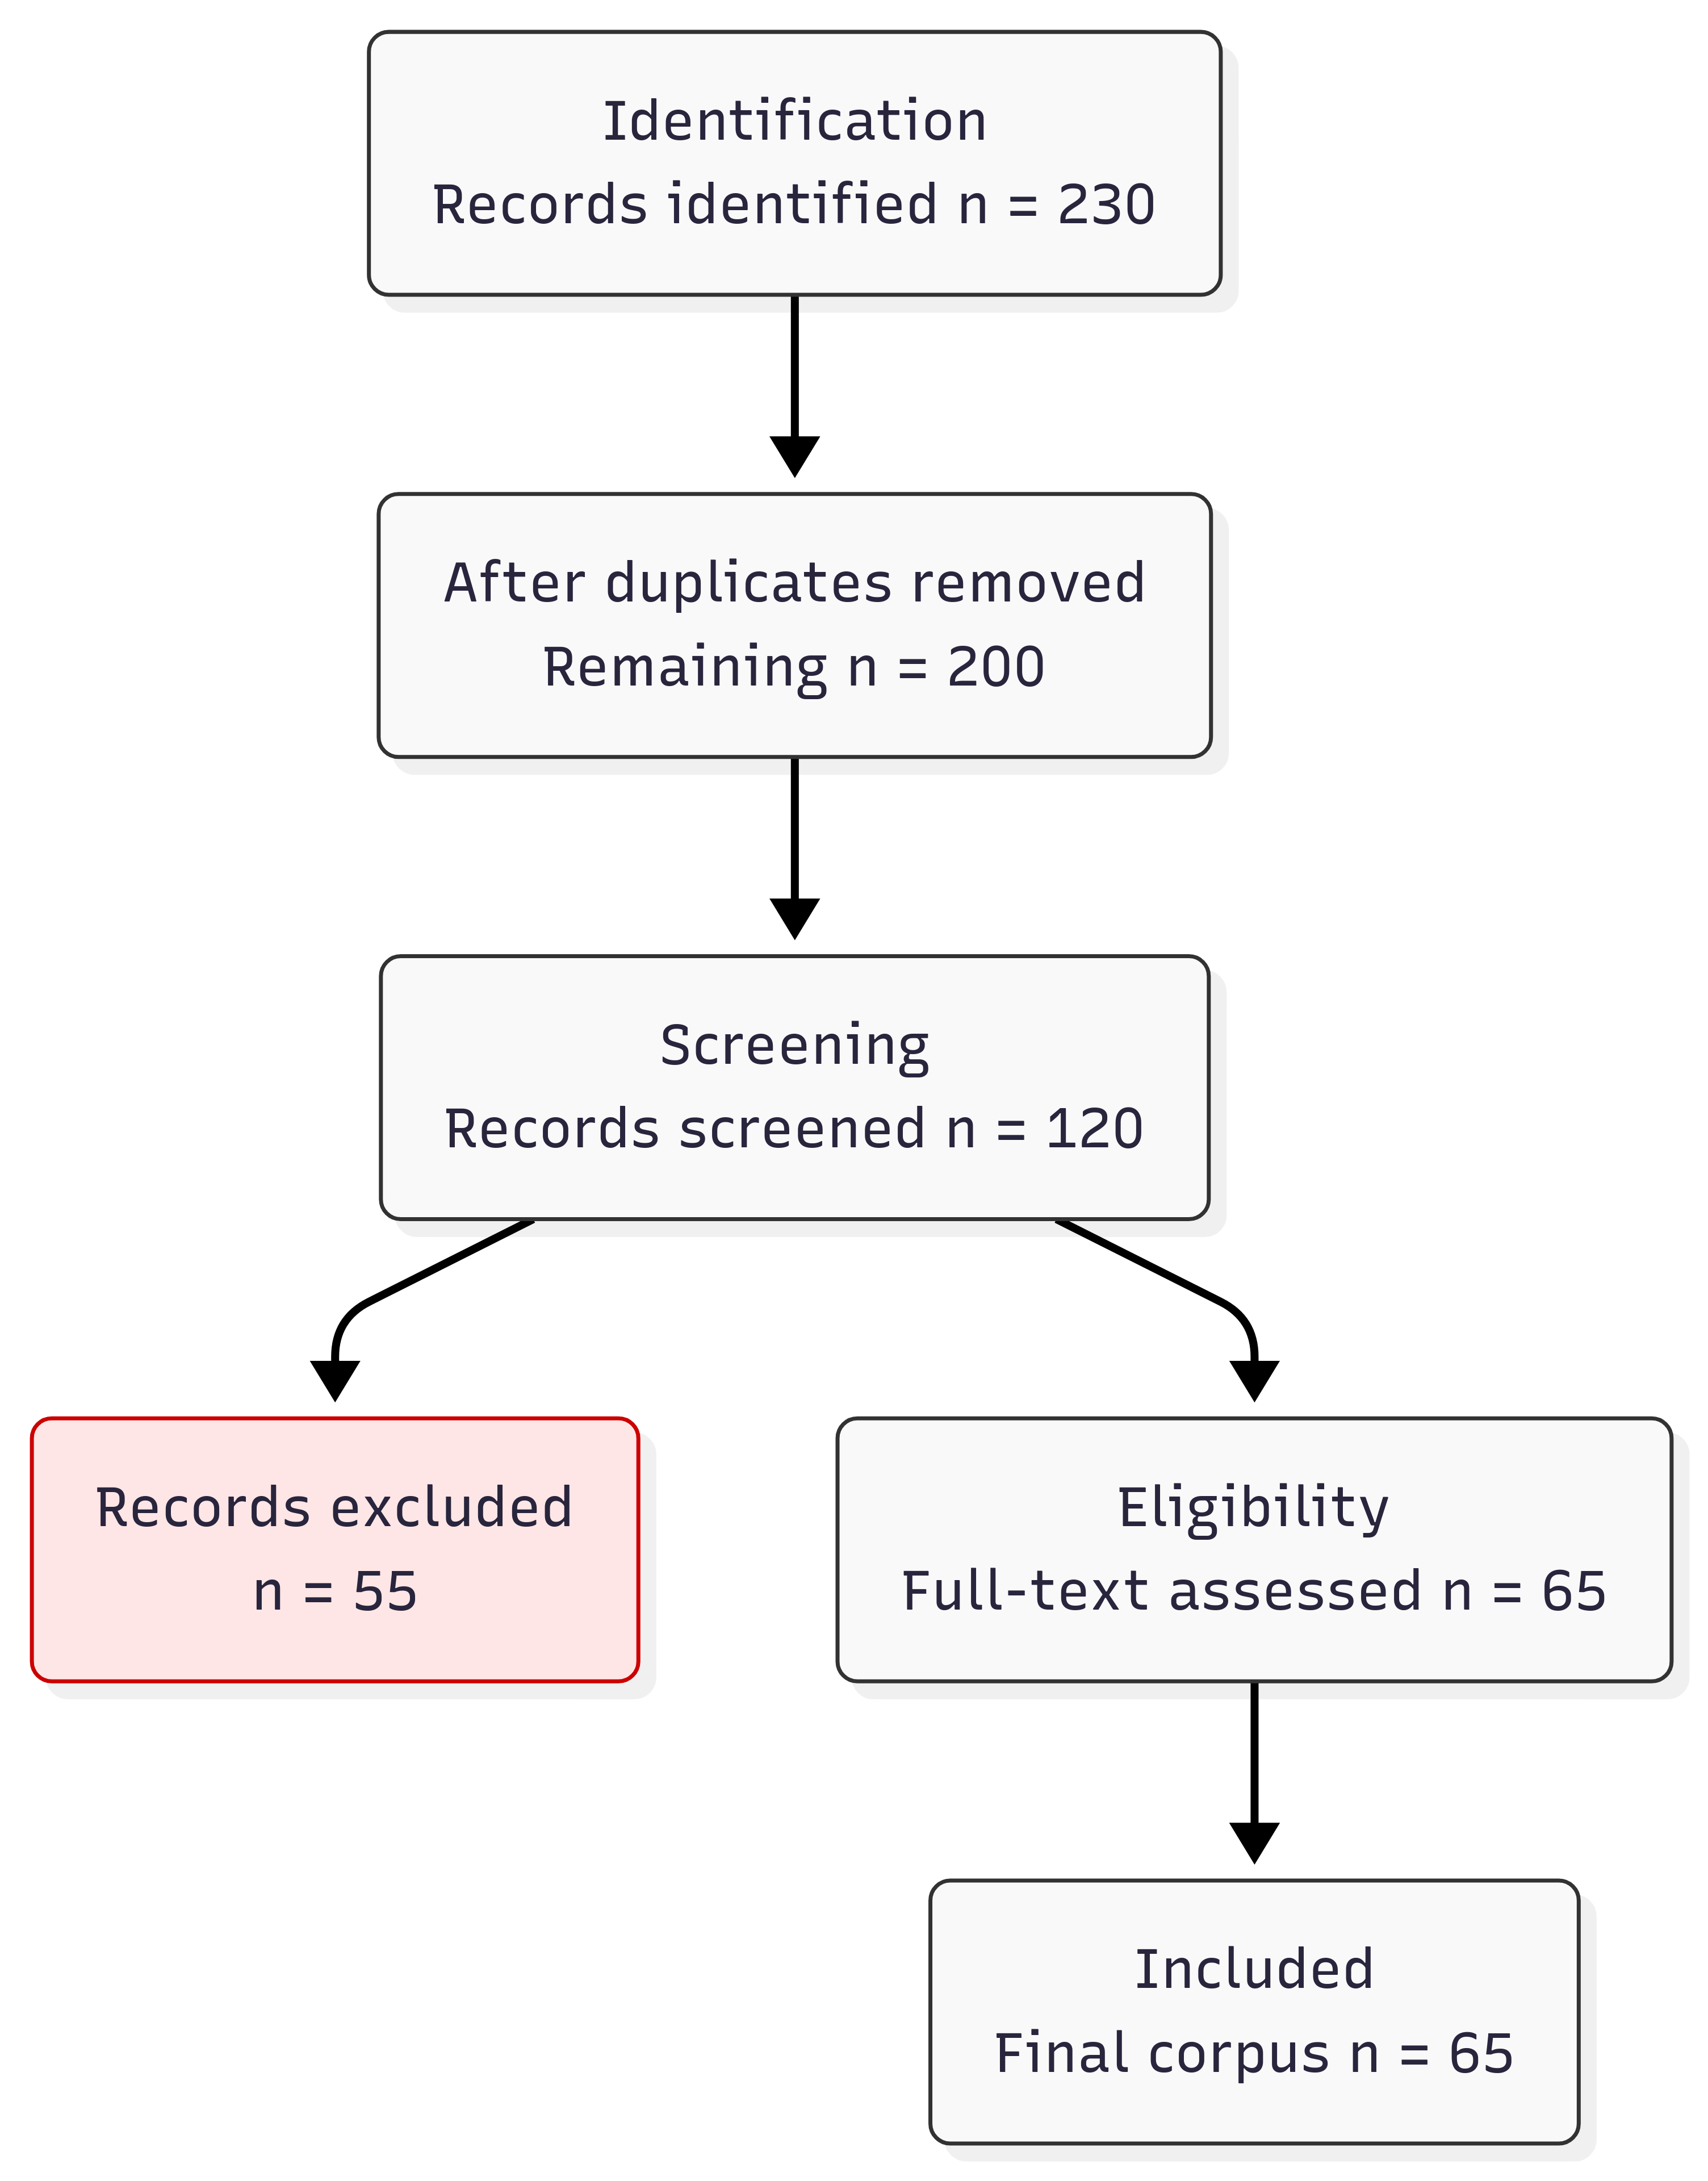
\includegraphics[width=0.8\textwidth]{src/fig/prop/06/prisma.png}
\caption{PRISMA flow diagram of document selection (final corpus $n=65$).}
\label{fig:prisma}
\end{figure}


\subsection*{Coding Protocol}
Documents are coded with a structured codebook:  
(1) Frames (diagnostic, prognostic, motivational),  
(2) Bricolage mode (layering, patching, transposition),  
(3) Uptake Index (0–4, + negative uptake, + timing).  

All coding decisions are memoed and version-controlled.

\subsection*{Reliability Strategy}
\begin{enumerate}
    \item Training round on 8–10 documents. 
    \item 25\% double-coded in both countries. 
    \item Cohen’s $\kappa$ reported (target ≥ 0.7). 
    \item Mid-project drift check + adjudication log. 
\end{enumerate}

\subsection*{Tools and Data Management}
Coding in \textbf{MAXQDA}, exported for transparency.  
Supplementary replicability checks in Python/R (text reuse detection, descriptive stats).  
All logs and metadata archived with version control.

\subsection*{Reflexivity and Safeguards}
\begin{itemize}
    \item Anonymized coding (first pass) to reduce reputational bias.  
    \item Adversarial memos: each bricolage instance paired with counter-interpretation.  
    \item Language awareness: coding in DE/ES; translation issues documented.  
\end{itemize}

The researcher’s dual background (Latin America + Europe) is both an asset and a 
risk; reflexive safeguards ensure this positionality informs interpretation 
without biasing coding.

\subsection*{Link to Hypotheses}
This design operationalizes H1–H3. Uptake distributions (H1/H2) are compared 
descriptively (medians, ranges, visualizations). Actor-type differences (H3) 
are shown via cross-tabulations. Results are stratified by venue type.  
The feedback loop in Figure~\ref{fig:causal} is treated as \emph{conceptual}: 
empirical analysis traces only the forward chain (frames $\rightarrow$ bricolage 
$\rightarrow$ uptake).
% ================================
% Conclusion
% ================================

\section*{Conclusion}
\addcontentsline{toc}{section}{Conclusion}

This thesis develops a comparative framework that links discursive institutionalism 
with ideational bricolage to explain forest adaptation governance. Its contribution 
is threefold: (i) a causal model specifying how institutional density and fragmentation 
shape bricolage strategies, (ii) an Uptake Index that operationalizes discursive 
influence through observable indicators, and (iii) a North–South comparative design 
that incorporates Chile alongside Germany, countering Eurocentric bias in the field.

The design is explicitly bounded: it relies on document analysis and captures uptake 
only as observable incorporation, not actor intentions. Future research using 
interviews or process-tracing would be required to validate strategic intent more 
directly. Within these limits, the framework offers a transparent and replicable 
approach that contributes both theoretically and methodologically to debates on 
adaptation governance.

Within these limits, the framework offers a transparent and replicable approach that 
contributes both theoretically and methodologically to debates on adaptation governance. 
It also lays a foundation for future PhD-level research, where interviews and process-tracing 
could build on this baseline to deepen causal inference.


\clearpage
% ================================
% Timeline
% ================================

\section*{Timeline}
\addcontentsline{toc}{section}{Timeline}

\begin{table}[h!]
\centering
\caption{Revised work plan (Oct 2024 -- Feb 2025)}
\label{tab:timeline}
\begin{tabular}{@{}p{3cm}p{3.5cm}p{8cm}@{}}
\toprule
\textbf{Phase} & \textbf{Dates (Approx.)} & \textbf{Tasks and Deliverables} \\ \midrule

\textbf{Phase I: Framework \& Corpus Setup} & Oct 2024 & 
Finalize revised proposal; build document archive (laws, reports, NGO briefs, media); define and lock coding scheme + Uptake Index. 
\textit{Deliverable:} Clean codebook + PRISMA figure. \\

\textbf{Phase II: Initial Coding \& Calibration} & Nov 2024 & 
Conduct conceptual pilot on 8--10 documents (Germany + Chile); adjust codebook after calibration; begin systematic coding of primary corpus (first 15--20 docs). 
\textit{Deliverable:} Memo + reliability check report. \\

\textbf{Phase III: Full Corpus Coding} & Dec 2024 -- mid Jan 2025 & 
Complete coding of remaining documents (aim: $\sim$40--50 total); draft descriptive summaries of Uptake Index patterns (by country, actor type); conduct robustness checks (weights, timing, negative uptake). 
\textit{Deliverable:} Draft of results tables + figures. \\

\textbf{Phase IV: Comparative Analysis \& Writing} & mid Jan -- early Feb 2025 & 
Write cross-case analysis (Germany vs Chile); draft propositions evaluation; write reflexivity and methodological safeguards. 
\textit{Deliverable:} Draft of Results + Discussion. \\

\textbf{Phase V: Finalization \& Submission} & Feb 2025 & 
Integrate supervisor feedback; finalize formatting and references; submit complete thesis. \\

\bottomrule
\end{tabular}
\end{table}

\paragraph{Feasibility note.}
The timeline is ambitious but feasible because the codebook and Uptake Index are already developed through preliminary document review. 
In practice, the corpus will be limited to approximately 40--50 documents, and phases of coding and memoing will partially overlap. 
This staggered design provides efficiency without sacrificing transparency, making completion by February 2025 realistic.
%
\section*{1. Abstract}
\addcontentsline{toc}{section}{1. Abstract}

This thesis examines how forest adaptation to climate change is governed in Germany and Chile. Using a comparative, discourse-centered approach, it applies the theoretical lenses of discursive institutionalism, ideational power, and institutional bricolage to explore the construction and legitimation of adaptation strategies. Drawing exclusively on primary/secondary sources---including legal frameworks, published policy strategies, and institutional narratives---it analyzes how responses to climate change emerge from the interplay of discourse and institutional architectures. The objective is to advance climate governance scholarship by connecting ideational dynamics with institutional practices in two high-profile, yet structurally distinct, political contexts.

\section*{2. Introduction}
\addcontentsline{toc}{section}{2. Introduction}

Forests are at once central to climate change mitigation and acutely threatened by shifting climatic patterns. Over the last decade, Germany and Chile have experienced frequent droughts, pest outbreaks, and declines in forest health; in Germany, four out of five trees were diagnosed as diseased in 2022 due to drought and insect infestations. Both countries are known to view forest governance as vital for meeting national and international climate goals.

This thesis investigates how contrasting institutional settings shape the discourse and practice of forest adaptation in Germany and Chile. By comparing these cases, the research seeks to reveal how divergent political traditions, actor coalitions, and institutional legacies affect adaptation responses. 

\textbf{Research Aim:}

The aim is to systematically compare how institutional architectures and discursive strategies condition forest adaptation governance in Germany and Chile---identifying both differences and points of convergence.

\textbf{Research Question:}

\begin{quote}
\textit{How do ideational power and institutional bricolage---within a discursive institutionalist framework---shape forest adaptation governance in Germany and Chile, and what insights does this comparison offer on the capacity of ideas and institutional flexibility to drive climate policy?}
\end{quote}

The research question focuses on three central concepts: (1) How actors use discourse and ideas to define and legitimize adaptation; (2) how institutional bricolage enables flexible, context-sensitive responses; and (3) whether discursive institutionalism can bridge cases with fundamentally different governance models. This approach not only identifies divergences and similarities, but also clarifies whether common theoretical frameworks are applicable across diverse contexts.

\section*{3. Literature Review}
\addcontentsline{toc}{section}{3. Literature Review}

\subsection*{3.1 Concepts and Definitions}

Discursive Institutionalism (DI) posits that ideas and discourse are central drivers of institutional change. Schmidt (2008, 2010) highlights both the coordinative role among elites and communicative function towards society. Ideational Power, developed by Carstensen and Schmidt (2016, 2018), describes actors' abilities to shape agendas and beliefs through discourse---via power over, and in ideas. Institutional Bricolage, pioneered by Cleaver (2001, 2012), theorizes how governance arrangements emerge from assembling existing institutional elements in context-sensitive ways, rather than relying solely on hierarchical design.

Underlying these concepts is the insight that institutional change in forest governance is often non-linear and responsive to ecological and social pressures. Connecting them enables analysis of how policy responses can be both institutionally embedded and discursively negotiated.

\subsection*{3.2 Status Quo of Research and Forest Governance}

Research on forest adaptation governance has grown rapidly since the mid-2010s. Early studies were dominated by technical adaptation frameworks and the study of policy instruments. More recently, there is recognition of the need to foreground institutional dynamics and actor discourse. Several reviews document how climate change is shifting forest sector priorities, while meta-analyses highlight ongoing challenges, including conflicting interests between climate protection, resource extraction, and the timber industry.

In Germany, large-scale forest inventories reveal a marked decline in timber and carbon stocks since 2017, and forests have ceased to serve as a net CO$_2$ sink---now acting as a source due to climate-related dieback and intensive harvest. In Chile, scholarship emphasizes institutional fragmentation between public agencies (CONAF, MMA), private actors, and REDD$^+$ mechanisms---with adaptation often framed in market terms. Despite multiple national strategies (DAS 2024 in Germany, ENCCRV in Chile), long-term implementation remains challenged by competing actor coalitions and shifting policy priorities.

However, much of the literature remains siloed either in technical policy analysis or theoretical institutional critique. Comparative, discourse-centered research---focusing on how adaptation is constructed and legitimated in differing contexts---is rare.

\section*{4. Methodology}
\addcontentsline{toc}{section}{4. Methodology}

\subsection*{Research Design}
A qualitative comparative case study, using Germany and Chile as critical cases. Selection is based on their sharply contrasting institutional architectures and parallel exposure to climate-induced forest vulnerabilities.

\subsection*{Data Sources}
Analysis will rely exclusively on secondary sources:

\begin{itemize}
  \item National adaptation strategies (DAS 2024, ENCCRV)
  \item Climate legislation (KSG, Ley Marco de Cambio Climático)
  \item REDD$^+$ documentation and benefit-sharing reports
  \item Reports and statistics from FAO, UNFCCC, World Bank, CONAF, BMEL, Thünen Institute
  \item Academic publications and media documents
\end{itemize}

\subsection*{Analytical Framework}
\begin{enumerate}
  \item \textbf{Discourse Analysis}: Identify dominant narratives, actor coalitions, and framing strategies.
  \item \textbf{Process Tracing}: Unpack institutional change events, focusing on shifts in adaptation policy.
  \item \textbf{Comparative Matrix}: Structure findings across governance paradigm, actors, instruments, and discourse.
\end{enumerate}

\subsection*{Theoretical Orientation}
The thesis synthesizes discursive institutionalism and comparative institutional theory to illuminate how ideational strategies and institutional flexibility drive adaptation in forestry. It offers new insight into whether and how discursive approaches can transfer across divergent institutional landscapes.

\section*{5. Timeline}
\addcontentsline{toc}{section}{5. Timeline}

\begin{longtable}{@{}ll@{}}
\toprule
\textbf{Month} & \textbf{Task} \\ \midrule
October 2025 & Finalize research design and literature review; begin coding scheme \\
November 2025 & Document analysis: Germany (laws, strategies, inventories) \\
December 2025 & Document analysis: Chile (ENCCRV, REDD$^+$, institutional reports) \\
January 2026 & Comparative analysis and synthesis of cases \\
February 2026 & Draft: Introduction, Methods, and Case Study chapters \\
March 2026 & Draft Discussion, Conclusions; editing and revision \\
April 2026 & Final proofreading, submission, and defense preparation \\
\bottomrule
\end{longtable}

%\input{src/chapters/00-proposition.tex}
%\input{src/chapters/00-plan.tex}
%\input{src/chapters/01-introduccion.tex}
%\input{src/chapters/02-marco-teorico.tex}
%\input{src/chapters/03-metodologia.tex}
%\input{src/chapters/04-resultados.tex}
%\input{src/chapters/05-discusion.tex}
%\input{src/chapters/06-conclusiones.tex}
% -------- Bibliografía --------

\printbibliography

\end{document}